\documentclass{beamer}

\usepackage{tikz}
\usepackage[labelfont=bf]{caption}
\usepackage{booktabs}
\usepackage{caption}
\usepackage{siunitx}
\usepackage{amsmath}
\usepackage{pgfplots}
\usepackage{pgfplotstable}

\title{Proving Conservation of Energy through relating Spring Potential and Kinetic Energy}
\author{Henry Oehlrich\and Chelsea Liao\and Shreyas Raychaudhuri}

\begin{document}
\maketitle

\begin{frame}
    \frametitle{Abstract}
\end{frame}

\begin{frame}
    \frametitle{Experiment Setup}
    \begin{figure}
        \centering
        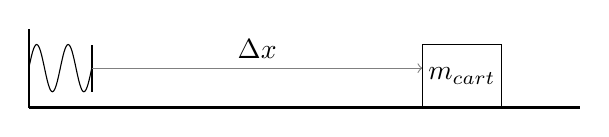
\begin{tikzpicture}
            \draw[thick] (0,0) -- (7,0);
            \draw[thick] (0,0) -- (0,1);
            \draw (0,0.5) sin (0.1,0.8) cos (0.2,0.5) sin (0.3,0.2) cos (0.4,0.5) sin (0.5,0.8)
                cos (0.6,0.5) sin (0.7,0.2) cos (0.8,0.5);
            \draw[thick] (0.8,0.2) -- (0.8,0.8);
            \draw[->,gray] (0.8,0.5) -- (5,0.5);
            \draw[rectangle,color=black] (5,0) rectangle (6,0.8) node[midway] {$m_{cart}$};
            \draw (2.9,0.5) node[above] {$\Delta x$};
        \end{tikzpicture}
    \end{figure}
    \begin{figure}
        \centering
        \begin{tabular}{l|l|l}
            \toprule
            Symbol & Description &  Value \\
            \midrule
            $m_{cart}$ & cart mass & \qty{0.286}{\kg} \\
            $k$ & spring constant & 0.75 \\
            $\Delta x$ & extension dist & varies \\
            $v$ & final velocity & measured \\
        \end{tabular}
    \end{figure}
\end{frame}

\begin{frame}
    \frametitle{Materials and Methods}
\end{frame}

\begin{frame} 
    \frametitle{Results} 
\end{frame}

\begin{frame}
    \frametitle{Discussion}
\end{frame}

\begin{frame}
    \frametitle{Acknowledgements}
\end{frame}

\end{document}
